% Left frame
%%%%%%%%%%%%%%%%%%%%
\begin{figure}
	\hfill
	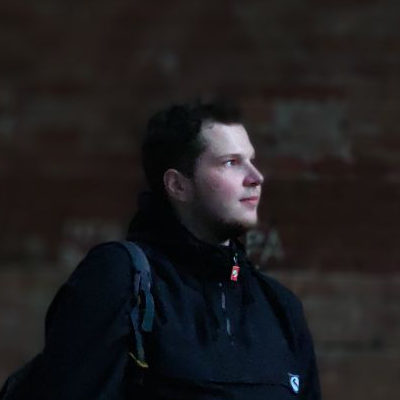
\includegraphics[width=0.6\columnwidth]{photo}
	\vspace{-7cm}
\end{figure}

\begin{flushright}\small

\end{flushright}\normalsize
\framebreak


% Right frame
%%%%%%%%%%%%%%%%%%%%
\Huge\bfseries {{\color{Cyan} Ilya} {\color{Black} Chesalin}} \\
\Large\bfseries Backend Developer \\

\normalsize\normalfont


\CVItem{Email} \url{ilya.chesalin@gmail.com}

\CVItem{Github} \url{github.com/evilyach}

\SmallSep

% About me
I was born in the ancient city of Ryazan, Russia and have been passionate about
information technologies for most of my life. Currently I am located in Moscow.

My professional interests span from programming to information security. I love
automating stuff around me to make my life easier, with technology being transparent
when I don't want or need it. I care about privacy, both personally and professinaly.


\Sep

% Skills
\CVSection{Skills}

\CVItem{Languages I speak}
\begin{multicols}{3}
\begin{compactitem}[\color{Cyan}$\circ$]
    \item Russian, native
    \item English, C1
    \item German, A1
\end{compactitem}
\end{multicols}

\SmallSep

\CVItem{Platforms}
\begin{multicols}{3}
\begin{compactitem}[\color{Cyan}$\circ$]
	\item Arch Linux
	\item Ubuntu / Debian
	\item macOS
	\item Windows with WSL
	\item \ldots
\end{compactitem}
\end{multicols}

\SmallSep

\CVItem{Programming and other Languages}
\begin{multicols}{3}
\begin{compactitem}[\color{Cyan}$\circ$]
    \item Python
    \item SQL
    \item Bash/Zsh
    \item \LaTeX
	\item \ldots
\end{compactitem}
\end{multicols}

\SmallSep

\CVItem{Technologies}
\begin{multicols}{3}
\begin{compactitem}[\color{Cyan}$\circ$]
    \item Open Source \heart\
    \item Flask
    \item FastAPI
    \item Git
    \item SQLAlchemy
    \item PostgreSQL
    \item Redis
    \item Celery
    \item Docker\{,-compose\}
    \item \ldots
\end{compactitem}
\end{multicols}

\Sep

% Experience
\CVSection{Experience}


\CVItem{November 2021 - present} \\
at \textit{Vizibl, UK}
as \textit{backend software engineer}
\SmallSep

After finishing university, I was looking for new opportunities. With my first
international team with people all around the world, we built b2b solution to
make our planet more sustainable and beautiful place to live.
\SmallSep

\texttt{macOS / Python / Flask / TDD / DDD / PostgreSQL / Docker}
\SmallSep


\CVItem{February 2020 - November 2021} \\
at \textit{SolidWall, Russia}
as \textit{backend software engineer}
\SmallSep

In February 2020 I joined a team of highly talented cybersecurity oriented
developers to perfect Web Application Firewall at SolidWall.
\SmallSep

\texttt{Linux / Python / PostgreSQL / Docker}
\SmallSep

\CVItem{October 2019 - February 2020} \\
at \textit{D-Link, Russia}
as \textit{full-stack software engineer}
\SmallSep

In October, I moved to another project, where I do full-stack web development.
\SmallSep

\texttt{Linux / JavaScript / NodeJS / VueJS / Quasar / MongoDB}
\SmallSep

\clearpage
\framebreak
\framebreak

\CVItem{November 2018 - September 2019} \\
at \textit{D-Link, Russia}
as \textit{embedded systems engineer}
\SmallSep

After taking cources on "Linux Embedded Programming Fundamentals" in
2017-2018, I got opportunity to join D-Link Developer team.
\SmallSep

\texttt{Linux / C / GDB / Valgrind}
\SmallSep

% Education
\CVSection{Education}
\CVItem{2016 - 2021} \\
at \textit{Ryazan State Radio Engineering University after V. Utkin}
\SmallSep

I have been a student at RSREU for 5 years, at the departament of Information Security of the Faculty of Computer Engineering. My speciality is Information Security of Automated Systems.

I have a Specialist's Degree with Honors in Information Security.

\SmallSep

\CVItem{2013 - 2016} \\
at \textit{Correspondence School of Physics and Technology of The Moscow Institute of Physics and Technology}
\SmallSep

Since ninth grade, I studied on programs of continuing education of a scientific and technical orientation.

\SmallSep

\CVItem{2005 - 2016} \\
at \textit{School 39 - Center of physical and mathematical eduation}
\SmallSep

At school I was passionate about mathematics and physics, taking part in lots of olympiads by Rosatom, MEPhI, URFO and many others.

\Sep

% Hackathons
\CVSection{Hackathons}

\CVItem{Hack.Moscow v3.0} \\
by \textit{Russian Hackers, Russia}
on \textit{25-27 October 2019}
\SmallSep

This was my first big hackathon, lasting 36 hours.

Our team decided to take Data Visualization track by Transparency
International. We came up with an idea that helps citizens to know their
officials in form of a game, that we called Chinder. We could not quite present
a polished product, but we had a lot of fun and gained a lot of experience.

\texttt{Java / Android Studio / Figma}

\SmallSep

\CVItem{Moscow Travel Hack 2020} \\
by \textit{Spinon, Russia}
on \textit{8-9 February 2020}
\SmallSep

My second big hackathon which took place before quarantine and lasted 30 hours.

Our team was chosen to take part in Discover Moscow's track to create service
to connect tourists with locals. During this hackathon, I was able to develop a
working Android application using VueJS and Cordova, and other members were
developing the beckend using Python and Flask.

\texttt{VueJS / Cordova / Quasar Framework / Figma}
